% vim:ts=4:sw=4
% Copyright (c) 2014 Casper Ti. Vector
% Public domain.

\chapter{系统设计}

\section{匹配算法设计}

\subsection{基本原理}
本文对于匹配算法的设计,主要的思想是探究出一种基于用户特征信息来推荐与用户志趣相投的人,所以其中必须要考虑到是现实用户对匹算算法实际效果的满意程度。之后对于不同的意见,对于匹配算法再进行不断对应的调整,从而得到一个相对最优的算法。故此,本文准备设计不同的匹配算法。最后对于不同的匹配算法进行实验,选取出实验效果最好的来当作最终实施在应用上的算法。
\subsection{基于人脸相似度的算法设计}

基于人脸相似度的算法设计的原理是提取用户提交的照片所提供的人脸特征,再将这一些特征与数据库中的图片的人脸特征结合起来,进行了基于算法的匹配。
face++的人脸识别所提供的特征值包括
\begin{enumerate}
\item 左眼和右眼在人脸上的相对坐标
\item 相应人脸的鼻尖在人脸上的相对坐标
\item 相应人脸的右侧嘴角和右侧嘴角在人脸上的相对坐标
\item 人脸的微笑程度分析结果,value的值为0-100的实数,越大表示微笑程度越高
\item 包含眼镜佩戴分析结果,value的值为None/Dark/Normal, confidence表示置信度
\end{enumerate}
假设一个用户提供的图片所显示的人脸为P,特征的维度为n,则用户的人靓可被定义为
\begin{equation*}
P=\{x_1,x_2,\ldots,x_n\}
\end{equation*}
设Face++提供的API的比较两张脸相似的算法为F,对于每个特征的损失函数为$L_i$,比较的人脸设为X,Y,则相似算法可表示为下式
\begin{equation*}
F=\sum_{i=1}^n L_i(x_i, y_i)
\end{equation*}
设本文的数据库的人脸集合为T,$T={T_1,T_2,\ldots}$,则我们能给出的基于人脸相似度的匹配结果的算法的公式如下
\begin{equation*}
G^{\*} = \mathop{\argmax_{G \in T}}{F(P,G)}
\end{equation*}

\subsection{机器学习算法设计}
由于基于人脸相似度的算法仅仅考虑了两个人脸特征的相似度,而基于一些美观上的经验,我们可以用过人脸的特征对于不同阶段不同年龄的人的审美进行机器学习,从而得到一个适合的算法。
但由于用户的不确定性,我们针对于用户的猜测可能导致负相关,因此这里的变量越少越好。由于现代人对于眼角位置的重视程度高于其他位置,而他们审美习惯基于自己的眼角相对位置。所以在这里本文使用了眼角位置作为我们的机器学习算法所学习的变量。
而这一个新的学习出的特征变量,我们将此当作一个新的权重加到之前之前基于人脸相似度的匹配算法上,从而达到优化匹配的目的,设r为该特征变量,则更新的匹配结果如下所示
\begin{equation*}
G^{\*} = \mathop{\argmax_{G \in T}}{\lambda * r+(1-\lambda)* F(P,G)}
\end{equation*}

本文将该机器学习问题看做一个分类问题(或一个监督学习问题),即根据用户本身图片的特征值和过去用户感兴趣的图片信息的历史特征值来对之后用户新提交照片的感兴趣的头像分类。

识别用户感兴趣的用户问题的目标是确定用户新提交的照片对应在数据库中的人脸的标签(即测试用例)。在以往用户点击的感兴趣的图片中,我们收集了一组过去的用户图片以及配对感兴趣的图片(即训练用例), 用D 表示这个集合。每个用例$d \in D$能被八个变量描述,即用户的左右眼角的相对坐标,和感兴趣的图片的人脸的左右眼角的相对坐标。

给定D和两张图片,一张图片为用户提供,一张图片为数据库提供,TapLock 系统需要确定密码的这一张数据库提供图片的标签 是用户感兴趣与否的。这里使用一个简化的 k-最近邻分类(k-Nearest Neighbor Classification,kNN)\parencite{ML1}\parencite{ML2}\parencite{ML3} 算法来解决这个问题。令 t 表示一个这两张图片的特征,去匹配在集合D中最近的向量。
\begin{enumerate}
\item 计算 t 和每个训练用例$d_{i} \in D$的距离,这里简化为笛卡尔距离
\item 选出距离值离 t 最近的训练用例$d_{1} \in D$。
\item 同样地,选出距离值𝛿离 t第二近的训练用例$d_{2} \in D$。
\item 如果两者标签相同,将选中的两个训练用例d1和d2的标签赋给 t。
\item 如果两者标签不相同 ,选出距离值离t 
第三近的训练用例$d_{3} \in D$,把d3的
标签赋给 t。
\end{enumerate}

\section{系统服务器架构设计}
本文设计了具有如下性质的社交应用好友匹配系统。系统的服务端包括了应用Face++API的SDK程序以及连接数据库持久化存储的媒介,为用户提供对应的服务接口,并且为应用维护者提供管理和维护其数据库的方法,为用户提供查询信息以及应用匹配算法的方法

\begin{figure}[h]
\centering
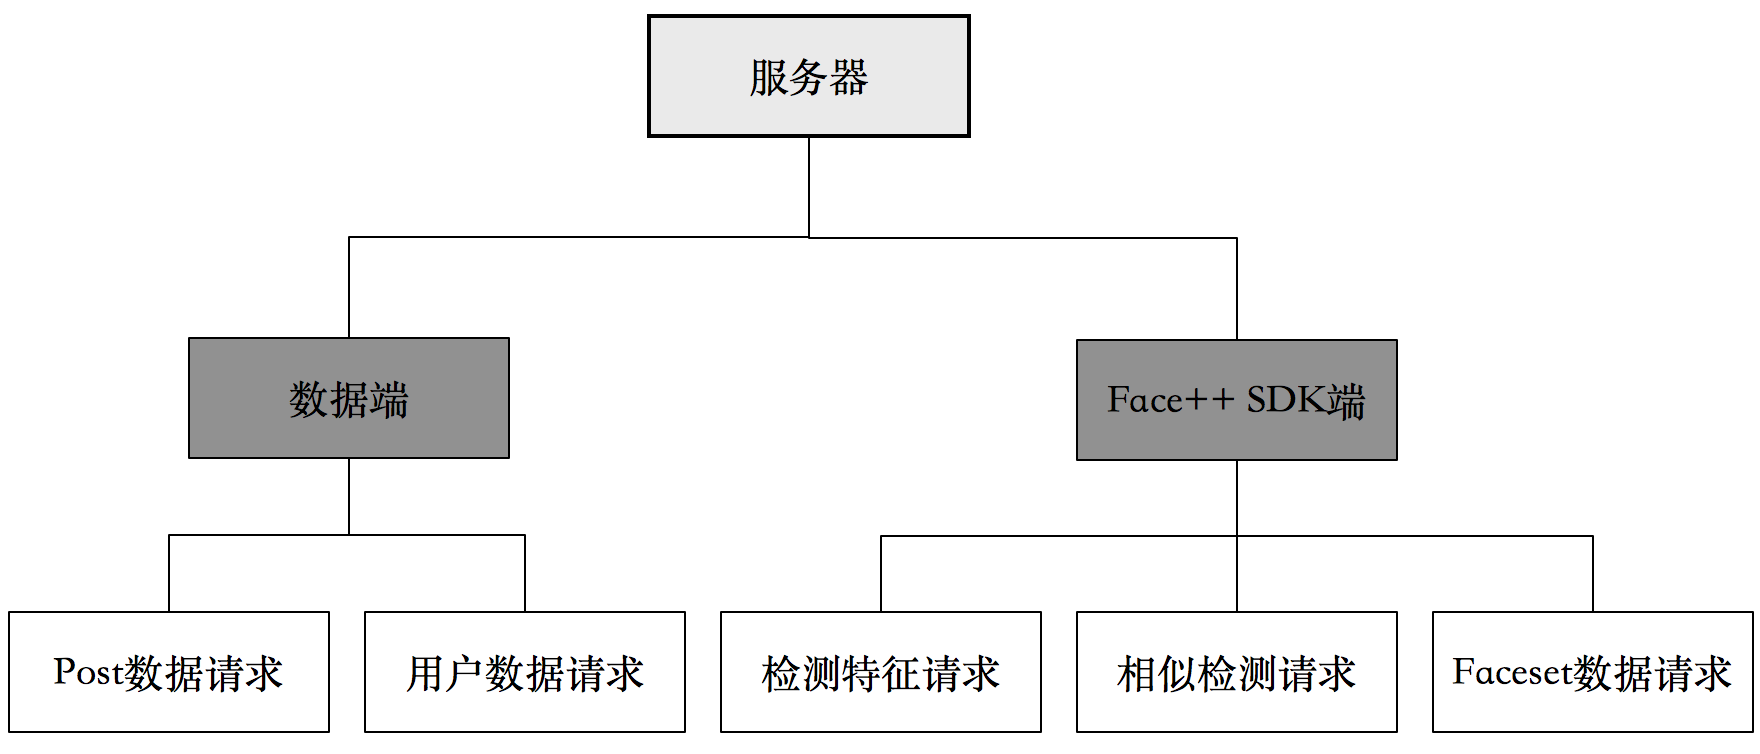
\includegraphics[width=\textwidth]{img/chap3/server.png}
\caption{服务器逻辑\label{Face++API}}
\end{figure}
 
图3.1描述了具体的服务器的逻辑,数据库端因为应用端实现了用户系统和人脸图片的post系统,所以在数据库这边的API上需要提供对应的连接到数据库的接口,从而使得我们能够在应用端展示出我们在数据库端的数据信息。

而Face++ API部分经过我们与应用端,匹配算法的协调,舍弃了一些原本需要的功能,比如Face++所提供的Group功能,而提供了与该系统相适应的4个请求接口。


\subsection{face++ SDK}
由于Face++并没有提供对应的SDK给node.js,所以本研究需要为face++的http请求的api实现一个SDK给node.js。

Face++的API可详见\parencite{face}

% \begin{figure}[h]
% \begin{minipage}[t]{0.45\linewidth}
% \centering
% 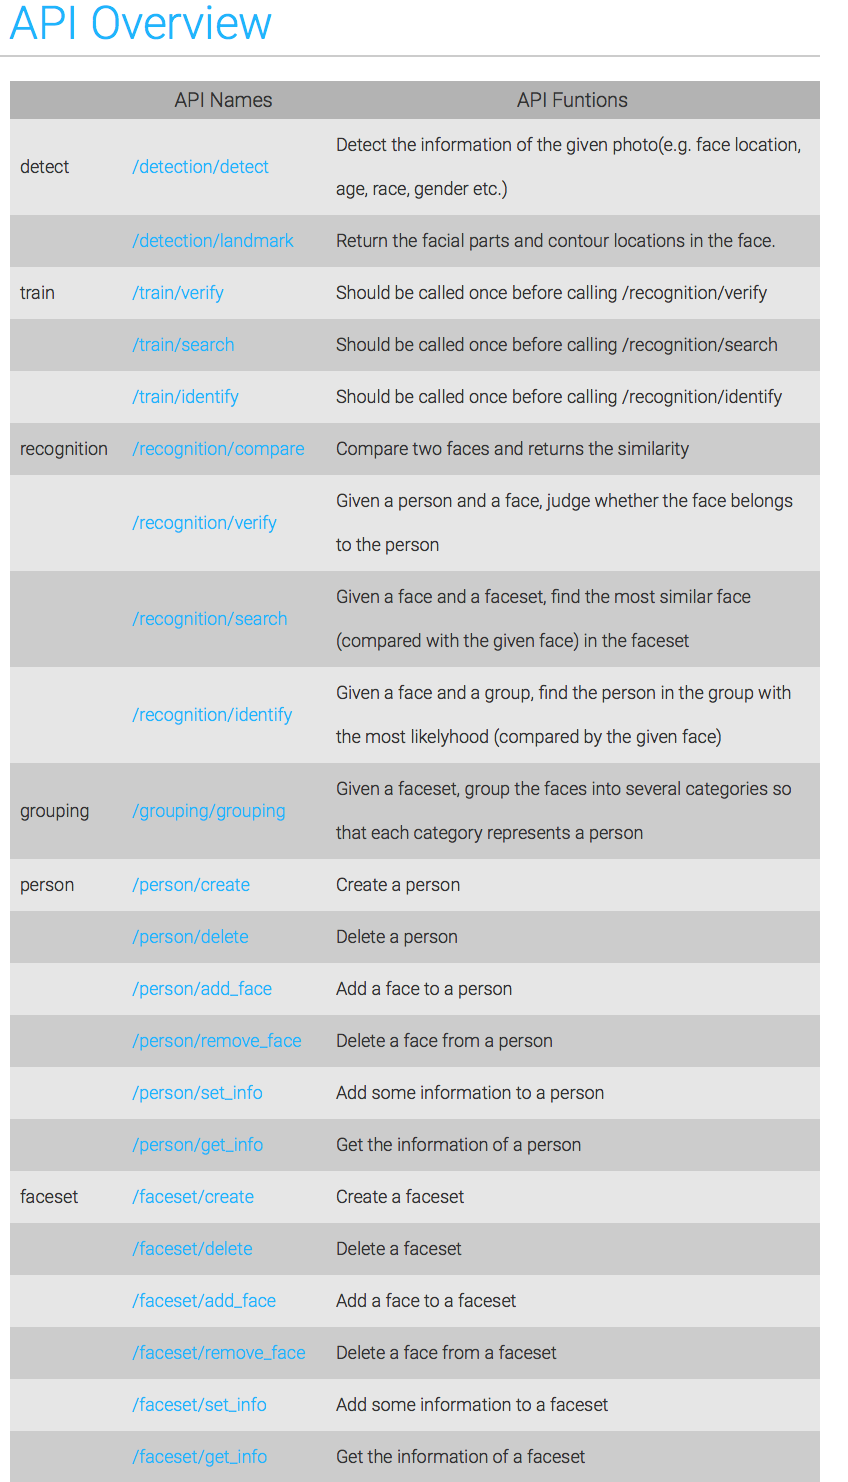
\includegraphics[width=\textwidth]{img/chap3/Face++API.png}
% \caption{Face++API\label{Face++API}}
% \end{minipage}
% \end{figure}
如何实现Face++API在nodejs上具体的SDK,因为和本文的研究关系不大,在此略过。

通过之前的描述,我们具体应用到的Face++的部分仅为face++ API的关于Detect,Compare,Face和FaceSet数据请求这方面的功能。

因此在实际的服务器端,对于我们完成的face++ SDK的这四个接口给以在服务器端的接口,使得我们的应用端在提交人脸图片已经进行匹配算法的时候可以利用Face++的人脸识别技术库完成我们需要的匹配算法模块。


\subsection{数据库}

为了完善我们的数据库的逻辑,因为NOSQL无法方便的进行系统的说明,故此本文对于数据库进行了用关系行数据库的描述对于NOSQL进行了比对。
\begin{figure}[h]
\centering
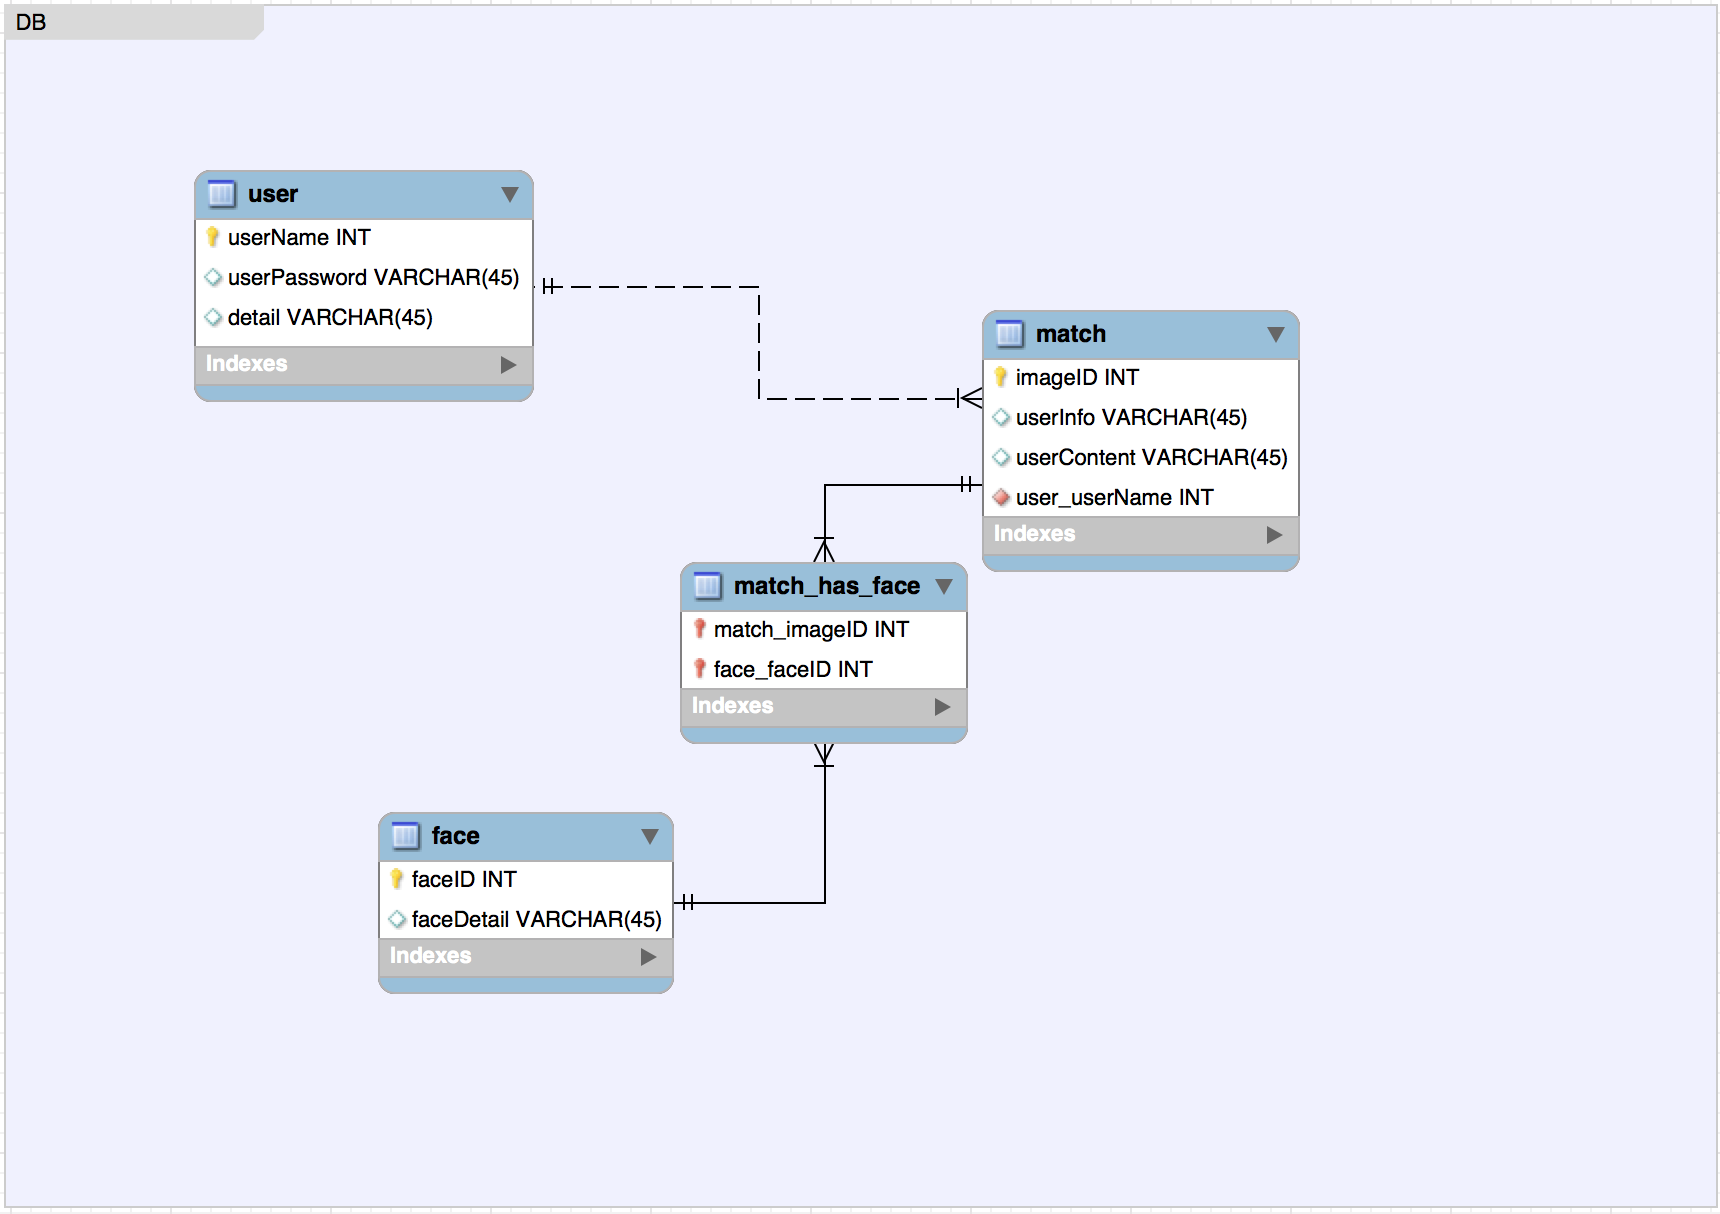
\includegraphics[width=\textwidth]{img/chap3/database.png}
\caption{关系型数据库表单抽象\label{Face++API}}
\end{figure}

图3.2表现了关系型数据库需要的表单,表现了三种需要表现的数据存储在数据库中,分别是用户信息,人脸信息,与对应的匹配信息。

经过我们数据库的逻辑和实际请求进行比对,我们发现服务器只需要实现post数据,用户获取数据以及更改的接口即可。






% 中文测试文字。


